\documentclass[aspectratio=169]{beamer}

\usetheme{metropolis}
\usepackage[T1]{fontenc}
\usepackage[utf8]{inputenc}
\usepackage{booktabs}
\usepackage{amsmath}
\usepackage{xcolor}
\usepackage{array}
\usepackage{graphicx}

\definecolor{lyapaxpurple}{HTML}{6D4AFF}
\definecolor{lyapaxdeep}{HTML}{2E1A47}
\definecolor{lyapaxmid}{HTML}{7C5CC4}
\definecolor{lyapaxsoft}{HTML}{EFE8FF}
\definecolor{lyapaxpale}{HTML}{FAF7FF}
\definecolor{lyapaxline}{HTML}{D8CBFF}

\setbeamercolor{background canvas}{bg=lyapaxpale}
\setbeamercolor{normal text}{fg=lyapaxdeep}
\setbeamercolor{frametitle}{fg=lyapaxdeep,bg=lyapaxsoft}
\setbeamercolor{title}{fg=lyapaxdeep}
\setbeamercolor{itemize item}{fg=lyapaxpurple}
\setbeamercolor{itemize subitem}{fg=lyapaxmid}
\setbeamercolor{block title}{fg=white,bg=lyapaxpurple}
\setbeamercolor{block body}{fg=lyapaxdeep,bg=white}
\setbeamercolor{callout}{fg=lyapaxdeep,bg=white}
\setbeamercolor{softbox}{fg=lyapaxdeep,bg=lyapaxsoft}
\setbeamercolor{accentbox}{fg=white,bg=lyapaxpurple}
\setbeamerfont{frametitle}{series=\bfseries,size=\large}
\setbeamertemplate{frametitle}{
  \vspace{0.15cm}
  \begin{beamercolorbox}[wd=\paperwidth,sep=0.22cm,leftskip=0.55cm]{frametitle}
    \insertframetitle
  \end{beamercolorbox}
}
\setbeamertemplate{navigation symbols}{}
\setbeamertemplate{itemize item}{\raise0.15ex\hbox{\scriptsize$\blacktriangleright$}}

\newcommand{\softbox}[1]{%
  \begin{beamercolorbox}[rounded=true,wd=\linewidth,sep=0.18cm]{softbox}
    #1
  \end{beamercolorbox}
}
\newcommand{\whitebox}[1]{%
  \begin{beamercolorbox}[rounded=true,wd=\linewidth,sep=0.18cm]{callout}
    #1
  \end{beamercolorbox}
}
\newcommand{\accentbox}[1]{%
  \begin{beamercolorbox}[rounded=true,wd=\linewidth,sep=0.20cm]{accentbox}
    #1
  \end{beamercolorbox}
}
\newcommand{\featurebox}[2]{%
  \whitebox{\textbf{#1}\par\vspace{0.05cm}{\small #2}}
}

\title{lyapax}
\subtitle{JAX-native Lyapunov spectra for ODEs, maps, networks, and DDEs}
\author{Abolfazl Ziaeemehr}
\date{}
\newcommand{\lyapaxversion}{v0.2.0}

\begin{document}

\begin{frame}[plain]
\vspace{0.75cm}
\begin{beamercolorbox}[rounded=true,wd=\linewidth,sep=0.45cm]{softbox}
{\Huge\textcolor{lyapaxpurple}{\textbf{lyapax}}}

\vspace{0.28cm}
{\Large JAX-native Lyapunov spectra}

\vspace{0.2cm}
{\large ODEs, maps, networks, and fixed-delay DDEs}
\end{beamercolorbox}

\vspace{0.55cm}
% \accentbox{\large Matrix-free tangent propagation with \texttt{jax.jvp} / \texttt{jax.vmap}}

\vfill
{\normalsize Abolfazl Ziaeemehr}

\vspace{0.08cm}
{\small Aix-Marseille University}

\vspace{0.18cm}
\begin{beamercolorbox}[rounded=true,wd=0.24\linewidth,sep=0.09cm,center]{softbox}
{\scriptsize version \lyapaxversion}
\end{beamercolorbox}
\end{frame}

\begin{frame}{Why another Lyapunov package?}
\softbox{\textbf{Computing Lyapunov spectra reliably is more than integrating a trajectory.}}

\vspace{0.35cm}

\begin{itemize}
  \item Propagate tangent directions alongside the state.
  \item Re-orthonormalize with QR over long horizons.
  \item Avoid forming dense Jacobians when only a partial spectrum is needed.
  \item Reuse the same machinery for custom models, networks, maps, and delay systems.
\end{itemize}

\vspace{0.25cm}
\accentbox{\textbf{Goal:} make Lyapunov-spectrum computation usable from ordinary JAX code.}
\end{frame}

\begin{frame}{What lyapax provides}
\begin{columns}[T,onlytextwidth]
\begin{column}{0.49\linewidth}
\featurebox{Systems}{ODEs, maps, coupled networks, and fixed-delay DDEs.}

\vspace{0.22cm}
\featurebox{Spectra}{Full spectra or leading partial spectra.}

\vspace{0.22cm}
\featurebox{Validation}{Examples against analytic, published, and independent-tool references.}
\end{column}
\begin{column}{0.49\linewidth}
\featurebox{JAX native}{Tangent propagation with \texttt{jax.jvp} and \texttt{jax.vmap}.}

\vspace{0.22cm}
\featurebox{Sweeps}{Batched parameters and initial conditions with \texttt{jax.vmap}.}

\vspace{0.22cm}
\featurebox{Backends}{CPU/GPU execution through JAX.}
\end{column}
\end{columns}
\end{frame}

\begin{frame}[fragile]{Minimal example}
\begin{block}{Lorenz spectrum}
\scriptsize
\begin{verbatim}
import jax
jax.config.update("jax_enable_x64", True)
import jax.numpy as jnp

from lyapax import lyapunov_spectrum, ode_problem, systems

rhs = systems.lorenz(sigma=10.0, rho=28.0, beta=8.0 / 3.0)
problem = ode_problem(rhs, state0=jnp.array([1.0, 1.0, 1.0]), dt=1e-2)

result = lyapunov_spectrum(
    problem, n_steps=50_000, renorm_every=10, t_transient=100.0
)
print(result.exponents)
\end{verbatim}
\end{block}
\end{frame}

\begin{frame}{Example output}
\whitebox{\centering
\includegraphics[width=0.88\linewidth]{../../docs/auto_examples/images/sphx_glr_03_chaotic_flows_001.png}
}

\vspace{0.08cm}
\softbox{\small Lorenz attractor and running Lyapunov-exponent convergence from the gallery examples.}
\end{frame}

\begin{frame}{Where it fits in the field}
\footnotesize
\whitebox{\textbf{\texttt{jitcode} / \texttt{jitcdde}}\par
Symbolic generation/compilation can dominate for dense large networks.}

\vspace{0.08cm}
\whitebox{\textbf{ChaosTools.jl}\par
Mature Julia ecosystem; Lyapunov workflow is CPU-oriented, not JAX/GPU-oriented.}

\vspace{0.08cm}
\whitebox{\textbf{Diffrax}\par
General JAX differential-equation solvers; no Lyapunov QR/tangent-spectrum API.}

\vspace{0.08cm}
\accentbox{\textbf{lyapax:} ordinary JAX models, matrix-free tangent propagation, partial spectra, sweeps, and DDE support.}
\end{frame}

\begin{frame}{Matrix-free scaling}
\begin{columns}[T,onlytextwidth]
\begin{column}{0.58\linewidth}
\whitebox{\centering
\includegraphics[width=0.88\linewidth]{../../docs/auto_examples/images/sphx_glr_10_matrix_free_scaling_001.png}
}
\end{column}
\begin{column}{0.39\linewidth}
\featurebox{Dense Jacobian}{Cost grows quickly when the full Jacobian is formed.}

\vspace{0.12cm}
\featurebox{\texttt{jvp}/\texttt{vmap}}{Track only the requested $k$ tangent directions.}

\vspace{0.12cm}
\featurebox{Target use case}{Partial spectra of large network models.}
\end{column}
\end{columns}
\end{frame}

\begin{frame}{GPU capability: the careful claim}
\begin{columns}[T,onlytextwidth]
\begin{column}{0.58\linewidth}
\whitebox{\centering
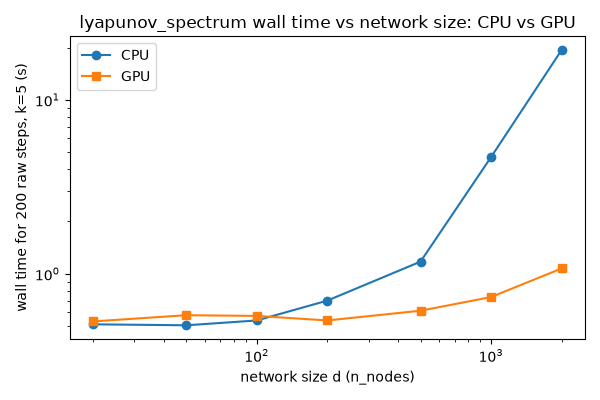
\includegraphics[width=\linewidth]{../../docs/_static/gpu_acceleration_reference.png}
}
\end{column}
\begin{column}{0.39\linewidth}
\accentbox{\textbf{GPU is not automatically faster.}}

\vspace{0.18cm}
\footnotesize
\begin{itemize}
  \item Small systems often run faster on CPU.
  \item GPU helps when arithmetic is large enough.
  \item Dense high-dimensional networks are the target case.
  \item Same JAX code can run on CPU or GPU.
\end{itemize}
\end{column}
\end{columns}
\end{frame}

\begin{frame}{Scaling snapshot}
\whitebox{
\begin{table}
\small
\begin{tabular}{>{\raggedleft\arraybackslash}p{0.23\linewidth}%
                >{\raggedleft\arraybackslash}p{0.18\linewidth}%
                >{\raggedleft\arraybackslash}p{0.18\linewidth}%
                p{0.27\linewidth}}
\toprule
Dense network size & lyapax CPU & lyapax GPU & Notes \\
\midrule
50   & 0.372 s  & 0.330 s & GPU near parity \\
200  & 1.075 s  & 0.265 s & GPU begins to pay off \\
1000 & 7.659 s  & 0.624 s & GPU clear win \\
2000 & 35.773 s & 1.419 s & GPU target regime \\
\bottomrule
\end{tabular}
\end{table}
}

\vspace{0.2cm}
\small
\softbox{Benchmark: dense Kuramoto network, partial spectrum with fixed $k=5$.
These numbers are a documentation snapshot, not a universal performance guarantee.}
\end{frame}

\begin{frame}{Good use cases}
\begin{columns}[T,onlytextwidth]
\begin{column}{0.49\linewidth}
\featurebox{Custom models}{JAX-defined ODEs and maps.}

\vspace{0.22cm}
\featurebox{Networks}{Coupled oscillator and dense network systems.}

\vspace{0.22cm}
\featurebox{Delay systems}{Fixed-delay DDEs with reusable Lyapunov machinery.}
\end{column}
\begin{column}{0.49\linewidth}
\featurebox{Large systems}{Partial spectra of high-dimensional states.}

\vspace{0.22cm}
\featurebox{Sweeps}{Parameter grids where JAX batching is useful.}

\vspace{0.22cm}
\featurebox{Research code}{Models close to NumPy-style Python.}
\end{column}
\end{columns}
\end{frame}

\begin{frame}{Scope and limitations}
\whitebox{\textbf{Focused package}\par
Not a general-purpose differential-equation solver.}

\vspace{0.18cm}
\whitebox{\textbf{ODE integration}\par
No implicit stiff ODE solvers in the core package. Adaptive ODE integration is available through Diffrax for tolerance control, not speed.}

\vspace{0.18cm}
\whitebox{\textbf{Delay and gradients}\par
DDE support is for fixed delays. Chaotic long-horizon gradients require care, even when autodiff runs.}
\end{frame}

\begin{frame}{Looking for feedback}
\accentbox{\Large\textbf{lyapax is usable now, and I am looking for real users.}}

\vspace{0.35cm}
\normalsize
\begin{itemize}
  \item Does the API fit how you define dynamical systems?
  \item Are the examples enough to get started?
  \item Which models should be added to the validation suite?
  \item Where does the package fail for your workflow?
\end{itemize}

\vspace{0.25cm}
\begin{columns}[T,onlytextwidth]
\begin{column}{0.31\linewidth}
\whitebox{\centering\texttt{pip install lyapax}}
\end{column}
\begin{column}{0.36\linewidth}
\whitebox{\centering\scriptsize\href{https://github.com/Ziaeemehr/lyapax}{\texttt{github.com/Ziaeemehr/lyapax}}}
\end{column}
\begin{column}{0.31\linewidth}
\whitebox{\centering\scriptsize\href{https://lyapax.readthedocs.io}{\texttt{lyapax.readthedocs.io}}}
\end{column}
\end{columns}
\end{frame}

\end{document}
